\chapter[Probabilistic Weighted Fuzzy Time Series]{Probabilistic Weighted Fuzzy Time Series} 
\index{Probabilistic Weighted Fuzzy Time Series}\index{PWFTS}
\label{chap:pwfts}

\newepigraph{Water is the softest thing, yet it can penetrate mountains and earth. This shows clearly the principle of softness overcoming hardness.}{Lao Tsu}

In this chapter proposes the basic  Probabilistic Weighted Fuzzy Time Series (PWFTS) method, a new FTS method for point, interval and probabilistic forecasting for one to many steps ahead. The PWFTS method aims to produce forecasts by dealing with two sources of uncertainty: fuzzy measurements and stochastic behavior. The fuzziness is induced for a data reduction purpose, in a process that reminds a simple bin discretization. The stochastic behavior is deduced by the  frequentist approach over the previous fuzzyfication. 

Regarding to Chapter \ref{chap:review_fts} fuzzy time series architectural chooses, the PWFTS method is a  time invariant and heuristic method to produce probabilistic weighted rules model $\model$. This method embodied all explored hyperparameters but their definition involves more complex optimization methods, that will be explored in Chapter \ref{chap:scalability}. Default values were defined for hyperparameters, except $k$ and $\Omega$ which must be determined by the user, as shown in Table \ref{tab:pwfts_hyperparam}. These values, however, can be overridden by user. 

\begin{table}[htb] 
    \centering
    \begin{tabular}{|c|c|} \hline
        \textbf{Parameter} & \textbf{Default Value}  \\ \hline
        $\Omega$ & User defined  \\ \hline
        $k$ & User defined  \\ \hline
        $\Pi$ & Grid \\ \hline
        $\mu$ & triangular  \\ \hline 
        $\alpha$-cut & 0 \\ \hline
        $L$ & $\{1,\ldots,\Omega\}$  \\ \hline
    \end{tabular}
    \caption{PWFTS hyperparameter default values}
    \label{tab:pwfts_hyperparam}
\end{table}

The option for a weighted rule knowledge model has the objective to help in the human readability and model explainability, also other knowledge extraction tasks. The weighted rule model will also help, as it will be seen in next chapters, in the distributed processing of the method and on its multivariate extension.

\index{Probabilistic Weighted Fuzzy Logical Relationship Groups}\index{PWFLRG}

The model rules (the Probabilistic Weighted FLRG's) describe the most probable future behavior (the $RHS$ - right hand side of the rule) given some past behavior (the $LHS$ - left hand side of the rule). For a given data sample there will be  many applicable rules with different activations (the membership weights) and all of them are taken into account.

The conception of this method mix the statistical approach of time series forecasting with the FTS techniques. Given some stochastic process $Y$, their best predictor is given by the conditional expectation $\mathbb{E}[y(t+1)\ |\ y(t),...]$. The FTS methods, especially that ones based on \cite{chen1996forecasting}, try to represent the behavior of $Y$ process by splitting their UoD in overlapping fuzzy sets, fuzzyfying the crisp data $Y$ to transform it on the fuzzy time series $F$ and identifying the sequential patterns.  The fuzzy sets are used to define zones, or fuzzy states, at the universe of discourse which have a common set of rules. That's what FLRGs really are: rules that describe sequential patterns. 

Then, for a given FLRG with form $LHS \rightarrow RHS$, where $F(t-1) = LHS$ and $F(t) \in RHS$ our best predictor can be rewritten from $\mathbb{E}[F(t+1)\ |\ F(t),...]$ to $\mathbb{E}[RHS|LHS]$.  The weights assigned to these rules are the frequentist probabilities of the fuzzy sets, measured during the training phase. 

Regarding the concepts introduced at Chapter \ref{chap:review_probforecasting}, the PWFLRG can be seen as a representation of a discrete empirical probability distribution.  The $RHS$ weights represent the conditional probability $P(A_i\ |\ LHS)$, $\forall A_i \in RHS$ and the $LHS$ weights represents the unconditional \textit{a priori} probabilities of the fuzzy sets. With the midpoints of each fuzzy set and their probabilities is possible then to compute the conditional expectation as a forecast for $F(t+1)$.

In next sections this mechanism is detailed, starting in Section \ref{sec:pwfts_empiricalprob} which discuss the basics of the fuzzy empirical probabilities. In Section \ref{sec:pwfts_training} the training procedure for first order model is presented, and on Section \ref{sec:pwfts_forecasting} the one step ahead method for probabilistic, interval and point forecasting is presented. Section \ref{sec:pwfts_extensions} presents extensions for high-order models and many steps ahead forecasting. On Section \ref{sec:pwfts_experiments} computational experiments are performed to asses the performance of the model and finally, on Section \ref{sec:pwfts_conclusion}, the main features of the proposed method are synthesized.  

%%%%%%%%%%%%%%%%%%%%%%%%%%%%%%%%%%%%%%%%%%%%%%%%%%%%%%%%%%%%%%%%%%%%%%
\section{Fuzzy Empirical Probabilities}
\label{sec:pwfts_empiricalprob}

%Given a univariate time series $Y(t) = \{y(0), y(1), ..., y(n)\}$, where $y(i) \in \mathbb{R}\ \forall i \in t$, $t \in [0, n]$ is the time index and the Universe of Discourse is defined by $U = [\min Y(t),\; \max Y(t)]$. Over $U$ is defined a linguistic variable $F$, with $p$ linguistic terms $A_i$ represented by overlapping fuzzy sets represented by their membership functions $\mu_{A_i}:\mathbb{R} \rightarrow [0,1]$.

%A Fuzzy Time Series $F(t)$ is a transformation of $Y(t)$ using the linguistic variable $F$. $F(t) = \{ f(0), f(1),..., f(n) \}$ where $f(i) = \{ \mu_{A_0}(y(i)), ..., \mu_{A_p}(y(i)) \}\ \forall i \in t$. $F(t)$ can also be represented by the linguistic values instead of the membership values, just by defining $f(i) = \{ A_k |  \mu_{A_k}(y(i)) > 0 \}\ \forall k \in [0,p]\ \forall i \in t$.

The core concept of PWFTS is the fuzzy empirical probability, used to compute the weights of the model, whose intuition is discussed in this section. The initial Zadeh's proposition of fuzzy probability, $P(A) = E[\mu_A]$, proposed in \cite{Zadeh1968}, demands the previous knowledge of the probability distribution over the universe of discourse. Once this distribution for $Y$ is unknown, an empirical distribution must take place. The simplest definition of empirical probability is the relative frequency of a discrete value or of a range of continuous values. Fuzzy Theory provides a different look at traditional Probability Theory because it affects the way the events are counted. On fuzzy sets the notion of event is more complex because the same value can belong to several sets with different degrees of membership, as shown in Figure \ref{fig:pwfts_fuzzyfrequency}. In that case, instead of accounting the integral (i.e. unary) occurrence of the event, their partial occurrence is accounted as the membership value. This method is known by fuzzy frequency, and was firstly  developed in \cite{Luo2000}. A related formulation can be found in \cite{Perfilieva2006}, with the concept of F-Transform, which decomposes the original domain of the time series into fuzzy frequencies over the fuzzy sets. This decomposition can also recreate the time series using the inverse transform. 

Given the sample space $U$ and the fuzzy sets $\ulvar$ over $U$, the partition function $Z_{\ufset}$, $\forall \ufset \in \ulvar$, is the integral of the membership function $\mu_{\ufset}$ over the sample space $U$, such that $Z_{\ufset} = \int_U \mu_{\ufset}(y) dy$ or the discrete approximation $Z_{\ufset} = \sum_{y \in U} \mu_{\ufset}(y)$. With the $Z_{\ufset}$ it is possible to approximate the empirical probability of a fuzzy set $\ufset \in \ulvar$ as the sum of its memberships $\mu_{\ufset}(y)$, $\forall y \in U$ divided by the sum of the partition functions $Z_{\ufset}$ of all fuzzy sets $\ufset \in \ulvar$, as presented in Equation \eqref{eqn:prob_conj_fuzzy}. 

\begin{equation}
P(\ufset) = \frac{\sum_{y \in U} \mu_{\ufset}(y)}{\sum_{\ufset \in \ulvar}Z_{\ufset}} 
\label{eqn:prob_conj_fuzzy}
\end{equation}

\begin{figure}
    \centering
    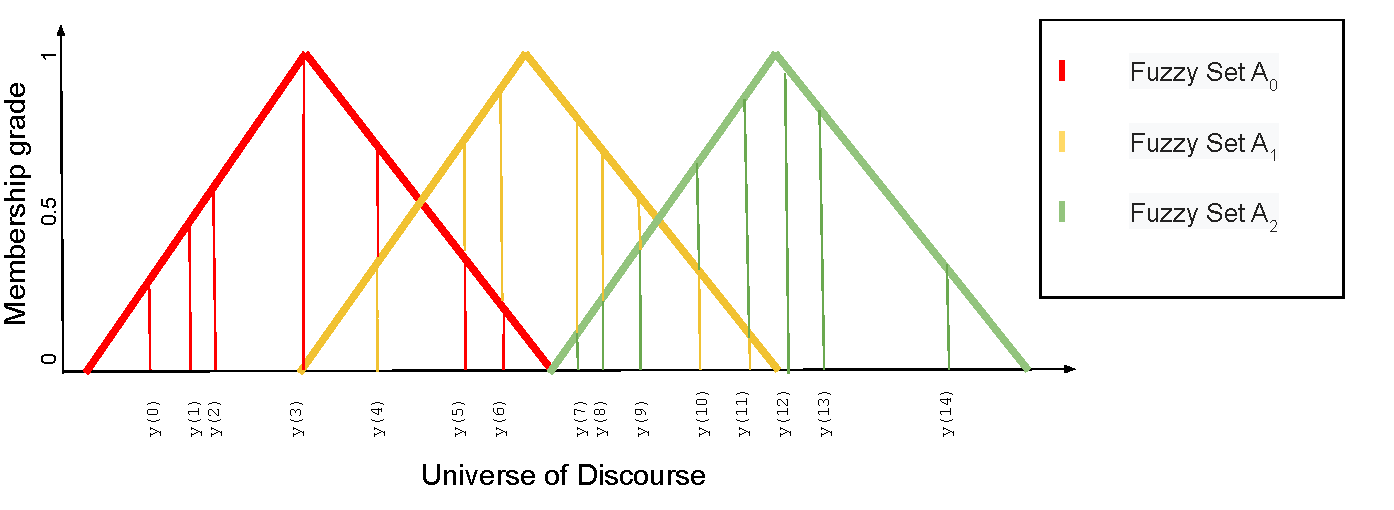
\includegraphics[width=\textwidth]{figures/pwfts_fuzzyfrequency.pdf}
    \caption{Fuzzy frequencies of each $y(t) \in Y$ used to approximate the fuzzy empirical probabilities $P(A_i)$ for each fuzzy set $A_i$}
    \label{fig:pwfts_fuzzyfrequency}
\end{figure}

The intuition behind this equation is that the empirical probability $P(\ufset)$ is evenly spread over the shape of the fuzzy membership function $\mu_{\ufset}$, and the point $y$ is a slice of this shape whose area is equal to the value $\mu_{\ufset}(y)$ (as shown in Figure \ref{fig:pwfts_fuzzyfrequency}), and the area of $\mu_{\ufset}$ is $Z_{\ufset}$. $P(A_i)$ is measured from a sample of $Y$, and this empirical value is an approximation of the true (but unknown) probability. This approximation is used in \eqref{eqn:prob_fuzzy} to approximate the conditional probability of a value $y \in U$, given a fuzzy set $\ufset \in \ulvar$:

\begin{equation}
P(y | \ufset) = P(\ufset) \cdot \frac{\mu_{\ufset}(y)}{Z_{\ufset}}
\label{eqn:prob_fuzzy}
\end{equation}

Using \eqref{eqn:prob_conj_fuzzy} and \eqref{eqn:prob_fuzzy} and the Law of Total Probability the empirical probability $P(y)$ can be approximated using the Equation \eqref{eqn:total_probability}. 

\begin{equation}
P(y,\ulvar) = \sum_{\ufset \in \ulvar} P(y | \ufset)\cdot P(\ufset)
\label{eqn:total_probability}
\end{equation}

The advantage of this approach is the convenience to obtain $P(\ufset)$ from a sample of the time series dataset $Y$. The accuracy of $P(\ufset)$ is determined mainly by $k$, the number of partitions of the universe of discourse $U$.


%%%%%%%%%%%%%%%%%%%%%%%%%%%%%%%%%%%%%%%%%%%%%%%%%%%%%%%%%%%%%%%%%%%%%%%%%%%%%%%%%
\section{PWFTS Training procedure}
\label{sec:pwfts_training}

The training procedure is a seven step method that learn the temporal dynamics of the time series training data $Y$ and represent it on a fuzzy-probabilistic model, namely the Probabilistic Weighted Fuzzy Temporal Rule - PWFTPG. The steps of the method are listed below :

\begin{enumerate}
\item[Step 1] \textit{Define the universe of discourse}: Define $U$ as the sample space of in-sample training data $Y$, such that $U = [\min(Y) - D_1, \max(Y)+D_2]$, where $[\min(Y), \max(Y)]$ is the range of in-sample data and $D_1$ and $D_2$ are numbers used to extrapolate this range, for instance $D_1 = 0.1\cdot\min(Y)$ and $D_2 = 0.1\cdot\max(Y)$;

\item[Step 2] \textit{Partitioning}: split $U$ in $k$ even length intervals $u_i$, for $i = 1,\ldots,k$, with midpoints $mp_i$;

\item[Step 3] \textit{Define the linguistic variable $\ulvar$}: Create $k$ overlapping fuzzy sets $\ufset$, with membership functions $\mu_{\ufset}$, related to an interval $u_j$, and midpoints $mp_j$. Each fuzzy set $\ufset \in \ulvar$ is a linguistic term of the linguistic variable $\ulvar$;

\item[Step 4] \textit{Fuzzyfication}: Transform the original numeric time series $Y$ into the FTS $F$, whose each data point $f(t) \in F$ is a $k$-tuple with the membership value of $y(t)$ with respect to each linguistic term $\ufset \in \ulvar$, such that:

\begin{equation}
f(t) = \left[\mu_{A_1}(y(t)),\ \mu_{A_2}(y(t)),\ \ldots,\ \mu_{A_k}(y(t)) \right]
\end{equation}

\item[Step 5] \textit{Generate the FTP set}: The Fuzzy Temporal Pattern - FTP\footnote{This nomenclature is adopted in replacement of Fuzzy Logical Relationships (FLR) used in \cite{song1993fuzzy}, to avoid misunderstandings with the terms ``logical" and ``relationship" with their classical meanings in fuzzy theory literature.} is a fuzzy rule with format $A_i \rightarrow A_k$ that indicates a temporal succession where the precedent (or the Left Hand Side - LHS) is $A_i \in f(t)$ and the consequent (or the Right Hand Side - RHS) is $A_k \in f(t+1)$, for each possible pair of $A_i \times A_k$ of membership values greater than zero, i.e.,  $\{A_i \rightarrow A_k\}$ $\forall A_i \in f(t)\ |\ \mu_{A_i}(y(t)) > 0$ and $\forall A_k \in f(t+1)\ |\ \mu_{A_k}(y(t+1)) > 0 $. . Therefore, $A_i \rightarrow A_k$ can be read as ``IF $y(t)$ is $A_i$ THEN $y(t+1)$ is $A_k$".
As each $f(t) \in F$ is a sparse $k$-vector of membership values, there will be many possible fuzzy sets combinations of two sequential vectors $f(t)$ and $f(t+1)$. Then for each sequential pair on $F$ possibly more than one FTP will be generated;

\item[Step 6] \textit{Generate the FTPG set}: A Fuzzy Temporal Pattern Group - FTPG\footnote{In replacement of Fuzzy Logical Relationship Group - FLRG used in \cite{Chen2006}.} represents the set of all FTPs with the same LHS and the union of their RHS, with the format $A_i \rightarrow A_k, A_j,...$, where the LHS is $f(t) = A_i$ and the RHS is $f(t+1) \in \{A_k, A_j,...\}$. Each FTPG can be understood as the set of possibilities which may happen at time $t+1$ (the consequent) when a certain set $A_i$ is identified at time $t$ (the precedent).

\item[Step 7] \textit{Calculate empirical probabilities}: The Probabilistic Weighted FTPG - PWFTPG adds weights on the LHS and the RHS that measure their fuzzy empirical probabilities. Each PWFTPG has the format $\pi_j \cdot A_j \rightarrow  w_{j0} \cdot A_0, ..., w_{jk} \cdot A_k$ for $j = 1,\ldots, k$. The set of all  PWFTPG, shown in \eqref{eqn:ftpg}, form the model $\model$. Its size depends on the number of partitions $k$, and it could be represented in matrix form but the weights $w_{ij}$ form a very sparse matrix, which justifies using optimized data structures for its representation.

\begin{equation}
\begin{array}{rcl}
\pi_1 \cdot A_1 & \rightarrow &  w_{11} \cdot A_1, ..., w_{1k} \cdot A_k \\
\ldots & \ldots & \ldots \\
\pi_k \cdot A_k & \rightarrow &  w_{k1} \cdot A_1, ..., w_{kk} \cdot A_k
\end{array}
\label{eqn:ftpg}
\end{equation}

Each weight $\pi_i$ is associated with the fuzzy set in the LHS of the rule, and it is the normalized sum of all LHS memberships of all FTPs where the LHS is the fuzzy set $\ufset$, as in \ref{eqn:prob_conj_fuzzy}. $\pi_i$ can be understood as the empirical \textit{a priori} probability of the fuzzy set $\ufset$ independent of time, or $P(\ufset)$, such that the condition of Equation \ref{eqn:apriori_condition} must be satisfied for the PWFTPG set in \ref{eqn:ftpg}.

\begin{equation}
    \sum_{j \in \ulvar} \pi_i = 1
    \label{eqn:apriori_condition}
\end{equation}

Each weight $w_{ji}$ is associated with a fuzzy set $\ufset$ on the RHS of the FTP whose the LHS is $\ufset$, and it is the normalized sum of all RHS memberships of all FTPs where $LHS = \ufset$ and $RHS = A_i$. Therefore, the weight $w_{ji}$ can be understood as the empirical conditional probability of the fuzzy set $A_i$ on time $t+1$ when the fuzzy set $\ufset$ is identified on time $t$, or $P(A_i^{t+1}\ |\ \ufset^t)$, such that the condition of Equation \ref{eqn:aposteriori_condition} must be satisfied for each $\ufset$ in LHS.

\begin{equation}
    \sum_{i \in \ulvar} w_{ji} = 1 \quad \forall \ufset \in \ulvar
    \label{eqn:aposteriori_condition}
\end{equation}


\end{enumerate}

The outcome of the Training Procedure is the PWFTPG set and it represents the temporal dynamics of the original data. It is an empirical probability distribution of the linguistic variable $A$ over the time series $Y$ with sample space $U$, where each rule contains the unconditional probability $P(\ufset) = \pi_j$ and conditional probabilities $P(A_i | \ufset) = w_{ji}$, for $A_i,A_j \in \ulvar$.

\begin{figure}
    \centering
    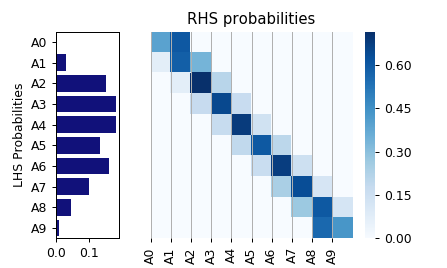
\includegraphics{figures/pwfts_rules_firstorder.png}
    \caption{Representation of first order PWFTPG ruleset}
    \label{fig:pwfts_rules_firstorder}
\end{figure}


%%%%%%%%%%%%%%%%%%%%%%%%%%%%%%%%%%%%%%%%%%%%%%%%%%%%%%%%%%%%%%%%%%%%%%%%%%%%%%%%%
\section{Forecasting Procedure}
\label{sec:pwfts_forecasting}

The forecasting procedure is a four step procedure listed in this section, which takes as input the forecasting type, a sample $y(t) \in U$ and uses the PWFTPG model $\mathcal{M}$ learned in the previous section to generate the output, which depends on the type of forecasting  (probabilistic, interval or point forecasting).  The complete forecasting procedure is presented below:

\begin{enumerate}
\item[Step 1] \textit{Fuzzyfication}: For a given input value $y(t) \in Y$, find the fuzzyfied values $f(t) = \{\ufset \ |\ \mu_{\ufset}(y(t)) > \alpha\}$;
\item[Step 2] \textit{Pattern matching}:  Locate all the PWFTPG's whose the LHS is $f(t)$.
\item[Step 3] \textit{Forecast}: The distribution of $f(t+1)$ is given by the RHS sets of each PWFTPG matched;
\item[Step 4] \textit{Defuzzyfication}: 
\begin{enumerate}
    \item If the forecasting type is Probabilistic, then build the probability distribution $P(y(t+1) | y(t))$, $\forall y(t+1) \in U$ applying Equation \ref{eqn:pwfts_probabilistic} presented in Section \ref{sec:pwfts_probabilistic};
    \item If the forecasting type is Interval, then build the prediction interval $\intvl(t+1)$ applying Equation \ref{eqn:pwfts_interval} presented in Section \ref{sec:pwfts_interval};
    \item If the forecasting type is Point, then build the crisp estimate $\estimate$ applying Equation \ref{eqn:pwfts_point} presented in Section \ref{sec:pwfts_point};
\end{enumerate}

\end{enumerate}


%%%%%%%%%%%%%%%%%%%%%%%%%%%%%%%%%%%%%%%%%%%%%%%%%%%%%%%%%%%%%%%%%%%%%%%%%%%%%%%%%
\subsection{Probabilistic Forecasting Procedure}
\label{sec:pwfts_probabilistic}

A probability distribution $P( y(t+1) | y(t))$, for all  $y(t+1) \in U$ can be computed using a Mixture Distribution approach to transform each PWFTPG probability into a continuous distribution, as described in Equation \ref{eqn:pwfts_probabilistic}.

A mixture distribution is defined as $P(y) = \sum \omega_j \cdot \pi_j(y)$ where $\pi_j: U \rightarrow [0,1]$ are specific PDFs and $\omega_j$ is a weight associated to each PDF, such that $\sum \omega_j = 1$. Given an input value $y(t) \in Y$ and the PWFTPG set, the probability distribution for each $y(t+1) \in U$ is given by \eqref{eqn:pwfts_probabilistic}, where $\omega_j$ is replaced by the probability $P(y(t)|A_i)$, the LHS probability given the input value, and the distribution $\pi_j$ is replaced by the probability $P(y(t+1)|A_j,A_i)$, $\forall A_j \in RHS$. 

Looking back to Equation \ref{eqn:prob_fuzzy}, it is clear that $\sum_{\ufset \in  \ulvar} P(y(t)|\ufset) < 1$, once $P(A_i)$ is the probability of the whole fuzzy set and $y(t)$ is just a small slice of it, thus it does not comply with the $\sum \omega_j = 1$ restriction of the mixture distribution. To work around this issue $P(y(t)|\ufset)$ is re-scaled using the Equation \ref{eqn:pwfts_rescaling}.

\begin{equation}
\frac{P(y(t)|\ufset)}{\sum_{\ufset \in \ulvar} P(y(t)|\ufset)}      
\label{eqn:pwfts_rescaling}
\end{equation}

Therefore, the final conditional probability $P(y(t+1) | y(t))$,  given the linguistic variable $\ulvar$ and a PWFTPG set $\model$, is defined in Equation \ref{eqn:pwfts_probabilistic}. A sample of the PWFTS probabilistic forecasting for one step ahead can be seen in Figure \ref{fig:pwfts_sample_manystep}.

\begin{equation}
\begin{array}{cl}
P(y(t+1) | y(t)) &=  \displaystyle \sum_{\ufset \in  \ulvar}\frac{\displaystyle P(y(t)| \ufset) \left( \sum_{i = 1}^k  P(y(t+1) | A_i,\ufset) \right)}{\displaystyle \sum_{i = 1}^k P(y(t)| A_i)}  \\
& \\
 &= \displaystyle \sum_{\ufset \in  \ulvar} \frac{ \displaystyle  \pi_j\frac{\mu_{\ufset}(y(t))}{Z_{\ufset}} \left( \sum_{i = 1}^k  w_{ji}\frac{\mu_{A_i}(y(t+1))}{Z_{A_i}} \right)}{\displaystyle \sum_{i = 1}^k \pi_i\frac{\mu_{A_i}(y(t))}{Z_{A_i}}}
\end{array}
\label{eqn:pwfts_probabilistic}
\end{equation}

\begin{figure}
    \centering
    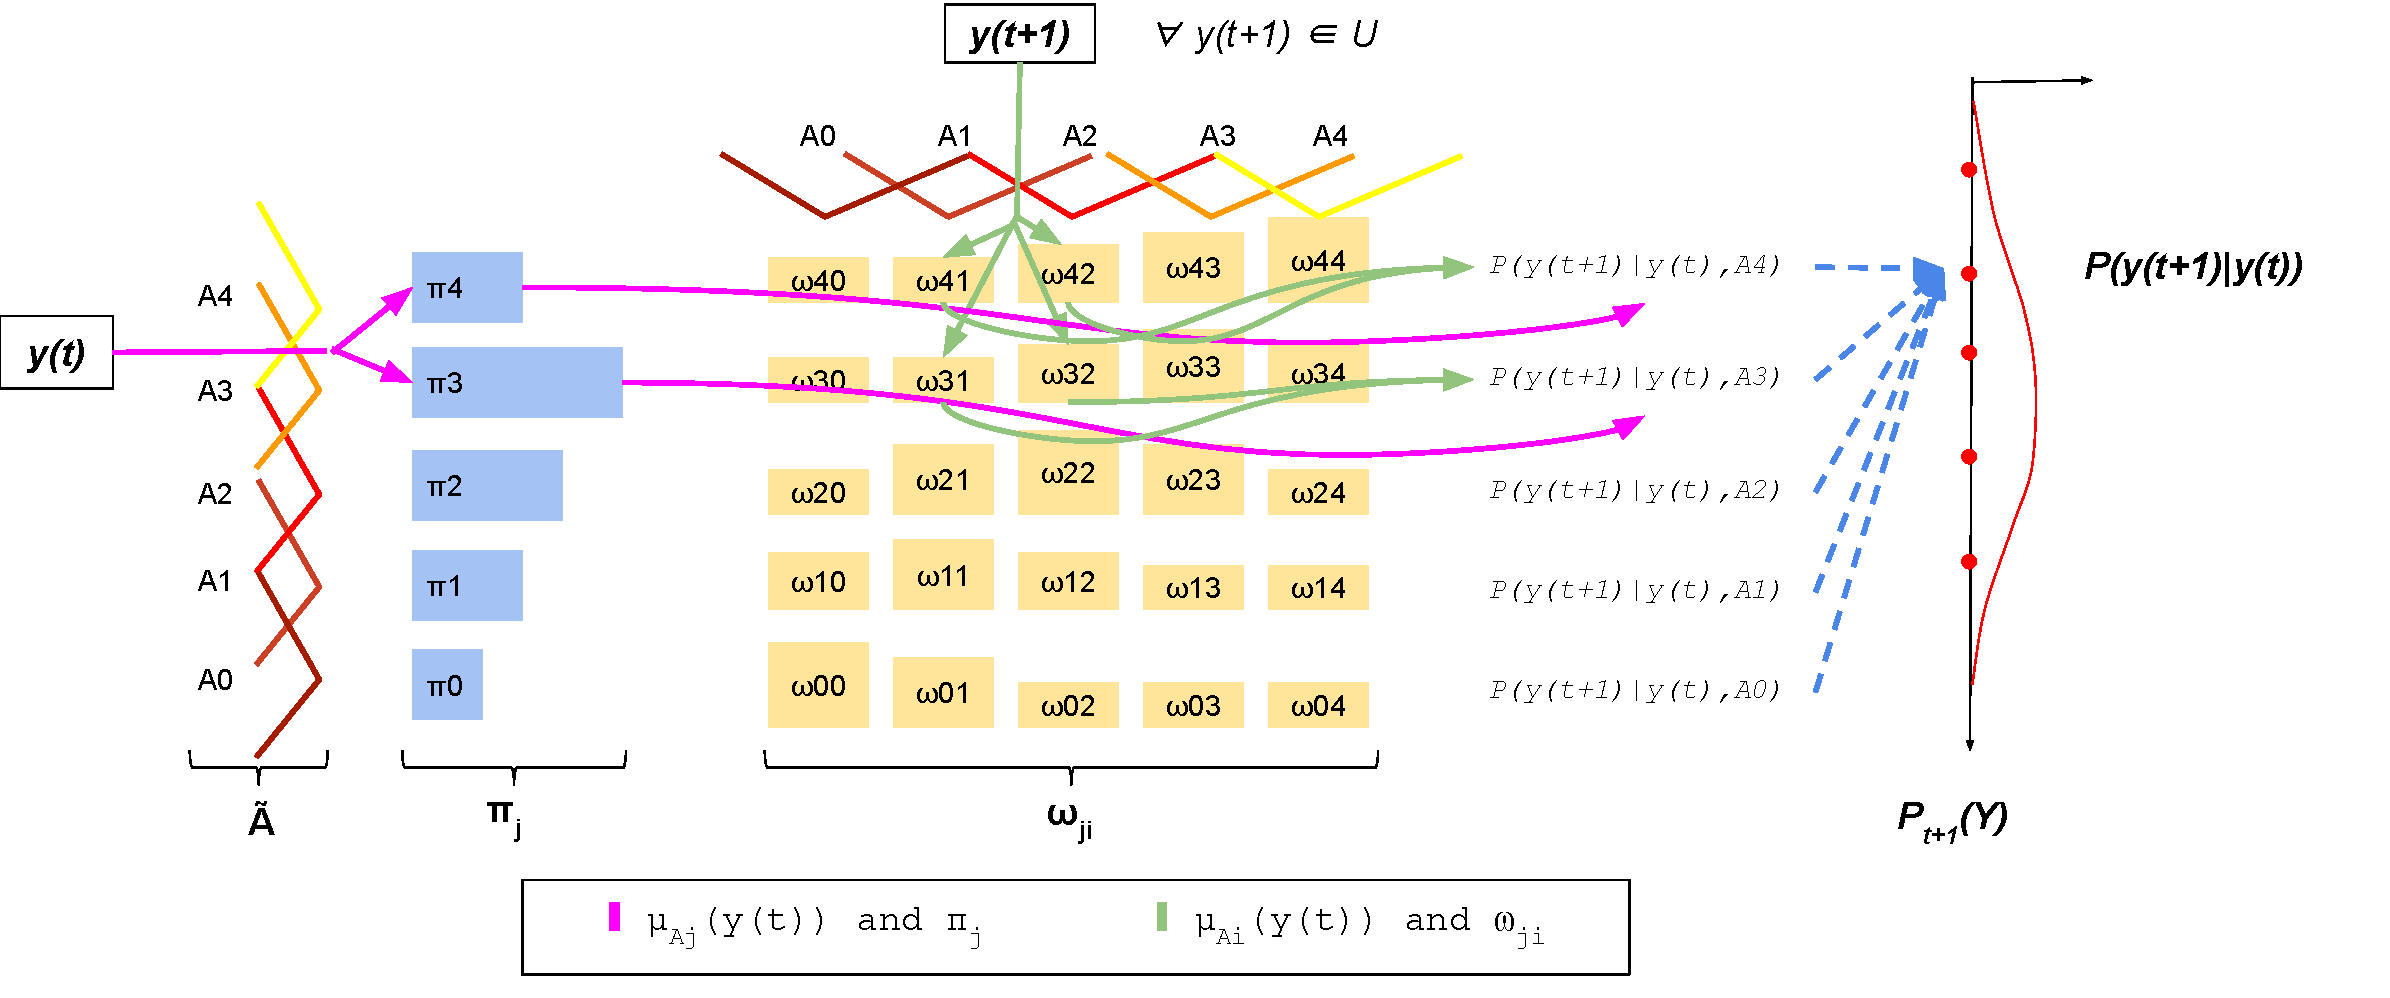
\includegraphics[width=\textwidth,height=7cm]{figures/pwfts_probabilistic_forecasting.pdf}
    \caption{Representation of PWFTS probabilistic forecasting procedure, where the length of blue boxes represents the magnitude of $\pi_j$ weights and the height of yellow boxes represents the magnitude of $\omega_{ji}$ weights.}
    \label{fig:pwfts_probabilistic_forecasting}
\end{figure}

\begin{figure}[htb]
    \centering
    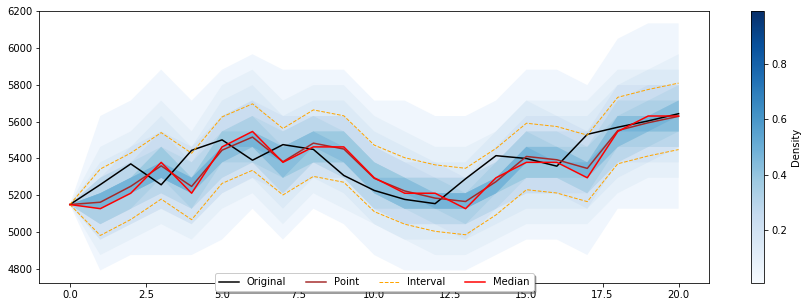
\includegraphics[width=\textwidth]{figures/pwfts_sample_onestep.png}
    \caption{Sample of PWFTS for one step ahead forecasting}
    \label{fig:pwfts_sample_onestep}
\end{figure}

\begin{figure}[htb]
    \centering
    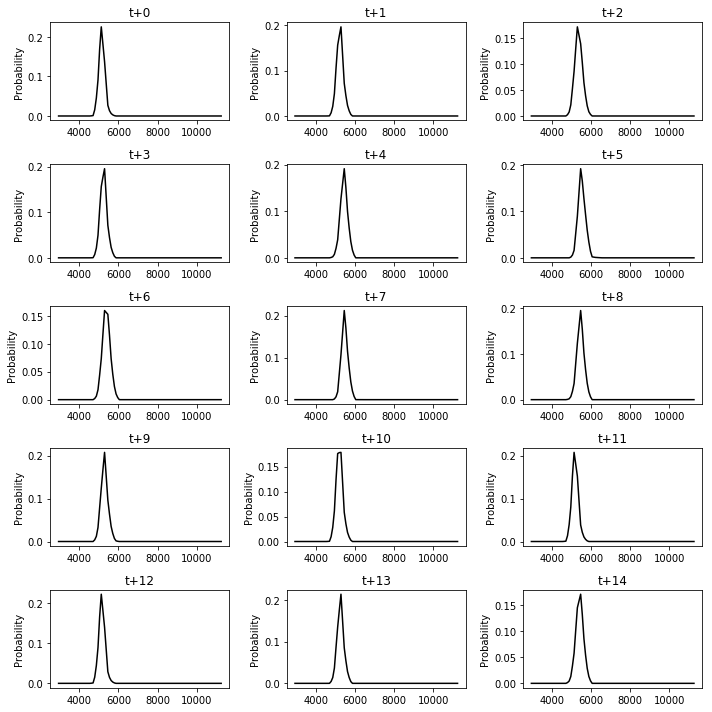
\includegraphics[width=\textwidth]{figures/pwfts_sample_onestep_tiled.png}
    \caption{Shapes of PWFTS probability distributions for one step ahead forecasting}
    \label{fig:pwfts_sample_onestep_tiled}
\end{figure}

%%%%%%%%%%%%%%%%%%%%%%%%%%%%%%%%%%%%%%%%%%%%%%%%%%%%%%%%%%%%%%%%%%%%%%%%%%%%%%%%%
\subsection{Interval forecasting procedure}
\label{sec:pwfts_interval}

A forecasting interval $\intvl (t+1)$ can be produced from $P( y(t+1) | y(t))$, once it is possible to build a cumulative density function $F( y(t+1) | y(t))$ and use it to construct the quantile function $Q(\tau): [0,1] \rightarrow U$, as shown in Equation \ref{eqn:quantile_function} where $\tau \in [0,1]$ is the desired quantile. Then, for a certain confidence level $\alpha \in [0,1]$, it is possible to compute an inter quantile interval $\mathbb{I}_f = [\underline{Q(\alpha)}, \overline{Q(1 - \alpha)}]$.

\begin{equation}
Q(\tau) = \min\{x \in U\ |\ F(x | y(t)) = \tau \}
\label{eqn:quantile_function}
\end{equation}

However, the above method demands the previous computation of the whole probability density function $P( y(t+1) | y(t))$, which is computationally expensive for larger input samples. A simpler and faster heuristic for generating prediction intervals extend the method $W\ifts$, proposed in Section \ref{sec:wifts}, to exploit the structure of the PWFTPG weights. Each PWFTPG will be represented by an interval $\intvl$ whose bounds are the expectation of the bounds of its RHS fuzzy sets, such that $\underline{\ufset}$ and $\overline{\ufset}$ represent the lower and upper bounds of the fuzzy set $\ufset$, and $\mathbb{E}[ \ufset ]$ is the expectation of the PWFTPG where the LHS is $\ufset$. The forecasting interval  $\intvl(t+1)$ then is the sum of these expectations weighted by the $P(y(t)|\ufset)$ probabilities, as presented in Equation \ref{eqn:pwfts_interval}. A sample of the PWFTS interval forecasting for one step ahead can be seen in Figure \ref{fig:pwfts_sample_manystep}.

\begin{equation}
\begin{array}{rcl}
\intvl_j & = & \displaystyle [\underline{\mathbb{E}[ \ufset ]}\ ,\ \overline{\mathbb{E}[ \ufset ]}] \\
\underline{\mathbb{E}[ \ufset ]} & = & \sum_{A_i \in \ufset^{RHS}} w_{ji}\cdot \underline{A_i} \\ 
\overline{\mathbb{E}[ \ufset ]} & = & \sum_{A_i \in \ufset^{RHS}} w_{ji}\cdot \overline{A_i}
\end{array}
\end{equation}

\begin{equation}
\begin{array}{rcl}
\mathbb{I}(t+1) & = & \displaystyle [\underline{\mathbb{E}[ \ulvar | y(t) ]}\ ,\ \overline{\mathbb{E}[ \ulvar | y(t) ]}] \\
& & \\
& = & \displaystyle \left[\frac{\sum_{\ufset \in \ulvar} P(y(t)|\ufset)\cdot \underline{\intvl_j}}{\sum_{\ufset \in \ulvar} P(y(t)|\ufset)},\frac{\sum_{\ufset \in \ulvar} P(y(t)|\ufset)\cdot \overline{\intvl_j}}{\sum_{\ufset \in \ulvar} P(y(t)|\ufset)}\right]
\end{array}
\label{eqn:pwfts_interval}
\end{equation}

%%%%%%%%%%%%%%%%%%%%%%%%%%%%%%%%%%%%%%%%%%%%%%%%%%%%%%%%%%%%%%%%%%%%%%%%%%%%%%%%%
\subsection{Point forecasting procedure}
\label{sec:pwfts_point}

To produce point forecasts $\estimate$ from the existing distribution $P(\cdot|y(t))$ it is only needed to apply the expectation operator, such that $\estimate = \mathbb{E}[P(y(t+1)|y(t))]$. This is also computationally expensive due to the computation of $P(y(t+1)|y(t))$. A simple heuristic for producing point forecasts is to compute the expectation $\mathbb{E}[\ufset]$ of each PWFTPG, as presented in Equation \ref{eqn:pwftpg_expectation}, where $mp_i$ is the midpoint of each fuzzy set $A_i \in RHS$. The expectation $\mathbb{E}[\ufset]$ for each PWFTPG $\ufset$ is constant and can be pre-computed. The final forecast $\estimate$ then is the sum of these expectations weighted by $P( y(t) | \ufset)$ probability, as shown in Equation \ref{eqn:pwfts_point}. A sample of the PWFTS point forecasting for one step ahead can be seen in Figure \ref{fig:pwfts_sample_manystep}.

\begin{equation}
\mathbb{E}[ \ufset ] = \displaystyle \sum_{i \in \ufset^{RHS}} w_{ji}\cdot mp_i
\label{eqn:pwftpg_expectation}
\end{equation}

\begin{equation}
\estimate = \displaystyle \mathbb{E}[ \ulvar | y(t) ] =  \sum_{\ufset \in \ulvar} \frac{ P(y(t) | \ufset) \cdot \mathbb{E}[ \ufset ]} { \sum_{\ufset \in \ulvar} P(y(t) | \ufset)}
\label{eqn:pwfts_point}
\end{equation}

%%%%%%%%%%%%%%%%%%%%%%%%%%%%%%%%%%%%%%%%%%%%%%%%%%%%%%%%%%%%%%%%%%%%%%%%%%%%%%%%%%%%%%%
%%%%%%%%%%%%%%%%%%%%%%%%%%%%%%%%%%%%%%%%%%%%%%%%%%%%%%%%%%%%%%%%%%%%%%%%%%%%%%%%%%%%%%%

\section{PWFTS extensions}
\label{sec:pwfts_extensions}

In the next subsections the basic first-order and one-step-ahead method is extended to higher orders and wider forecasting horizons in order to increase PWFTS method flexibility and versatility.

%%%%%%%%%%%%%%%%%%%%%%%%%%%%%%%%%%%%%%%%%%%%%%%%%%%%%%%%%%%%%%%%%%%%%%%%%%%%%%%%%%%%%%%
\subsection{Many steps ahead forecasting}
\label{sec:pwfts_many_step}

The forecasting procedures listed in Section \ref{sec:pwfts_forecasting} are one step ahead methods. To extend the forecasting procedures to many steps ahead forecasting, an iterative approach is adopted, in which the $t+1$ step is computed with the previously presented methods and its output is fed back as input to the next $H$ steps. From the step $t+2$ on, let $h \in [t+2, t+H]$ be the new time indexer. The simpler approach is to perform the point forecast of $y(h+1)$  with the input $y(h)$.

The interval procedure requires a few more modifications. Given the input $\intvl(h)$ the same interval forecasting procedure will be executed with inputs $\underline{\intvl(h)}$ and $\overline{\intvl(h)}$ producing two new intervals $\underline{\intvl(h+1)}$ and $\overline{\intvl(h+1)}$. Then the final forecasting interval will be $\intvl(h+1) = [\min\{\underline{\intvl(h+1)}\}, \max\{\overline{\intvl(h+1)}\}]$. 

Finally, the probabilistic forecasting for $P(y(h+1)|y(h))$ given the input will change to  \ref{eqn:extension_probabilistic}, instead of \ref{eqn:pwfts_probabilistic}. This equation replaces $P(y(h) | \ufset)$ for the previous probability distribution $P(y(h)|y(h-1))$. A sample of the PWFTS many steps ahead forecasting can be seen in Figure \ref{fig:pwfts_sample_manystep}.

%\begin{equation}
%\medmath{
%P(y(s+1) | y(s))  = \frac{\sum_{i = 1}^k %P(y(s)| y(s-1))\cdot \left(  \sum_{j = 1}^k  %P(y(s+1) | A_j,A_i) \right)}{\sum_{i = 1}^k %P(y(s)| y(s-1))}}
%\label{eqn:extension_probabilistic}
%\end{equation}

\begin{equation}
P(y(h+1) | y(h))  = \displaystyle \sum_{\ufset \in \ulvar} \frac{ P(y(h)| y(h-1), \ufset)}{ \sum_{i = 1}^k P(y(h)| y(h-1), A_i)} \times  \left(  \sum_{z = 1}^k  P(y(h+1) | A_z,\ufset) \right)
\label{eqn:extension_probabilistic}
\end{equation}

\begin{figure}
    \centering
    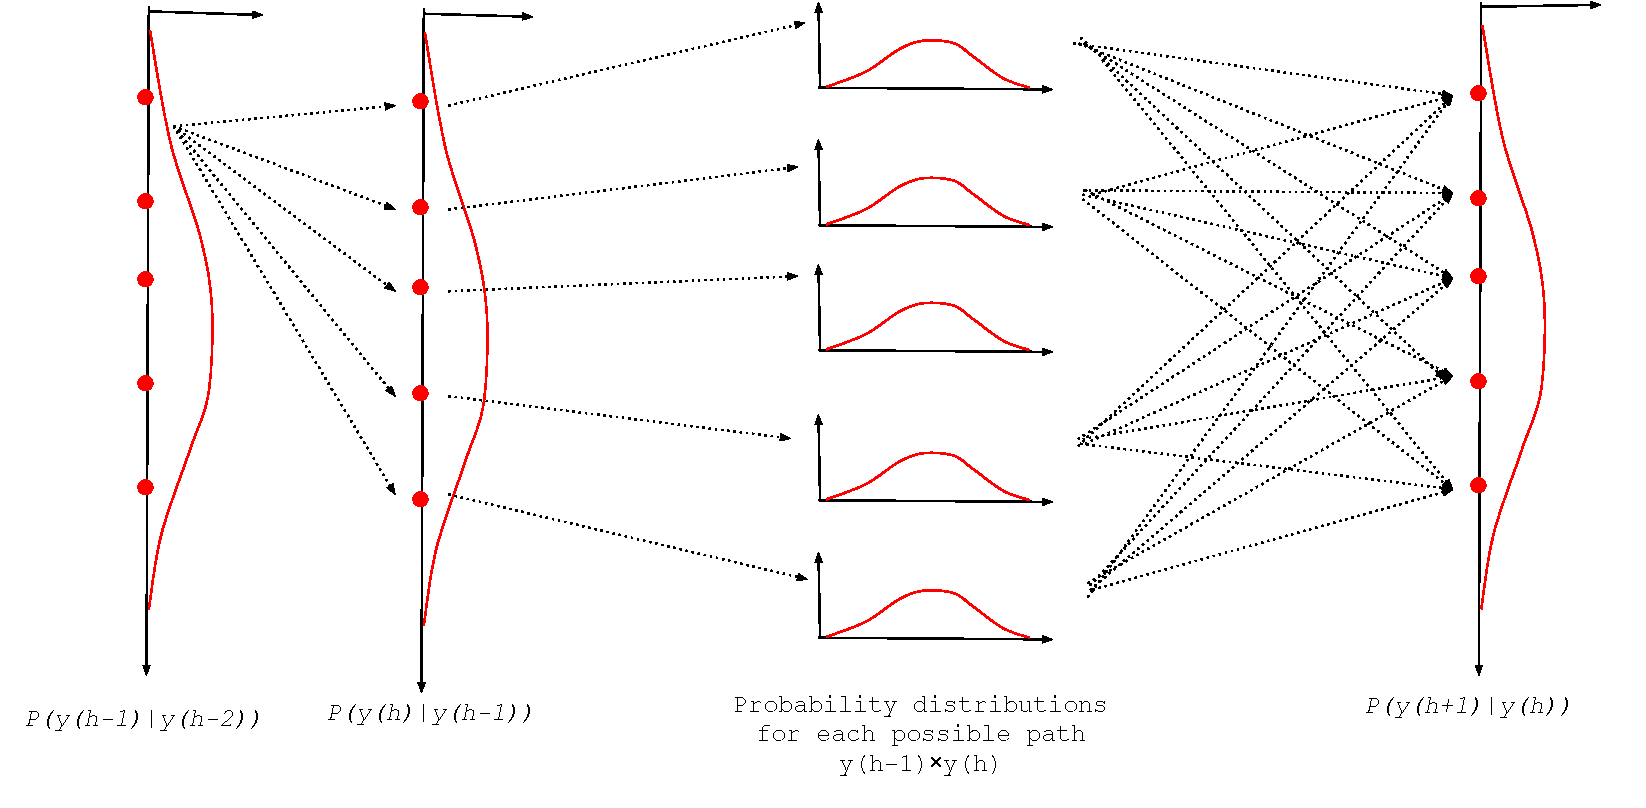
\includegraphics[width=\textwidth]{figures/pwfts_probabilistic_manysteps.pdf}
    \caption{Caption}
    \label{fig:pwfts_probabilistic_manysteps}
\end{figure}
 
\begin{figure}[htb]
    \centering
    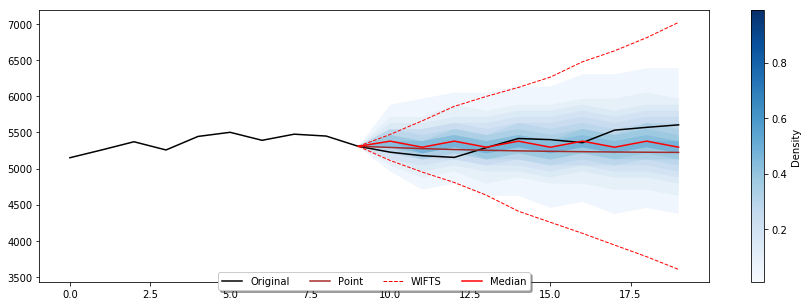
\includegraphics[width=\textwidth]{figures/pwfts_sample_manystep.png}
    \caption{Sample of PWFTS for 7 step ahead forecasting}
    \label{fig:pwfts_sample_manystep}
\end{figure}

\begin{figure}[htb]
    \centering
    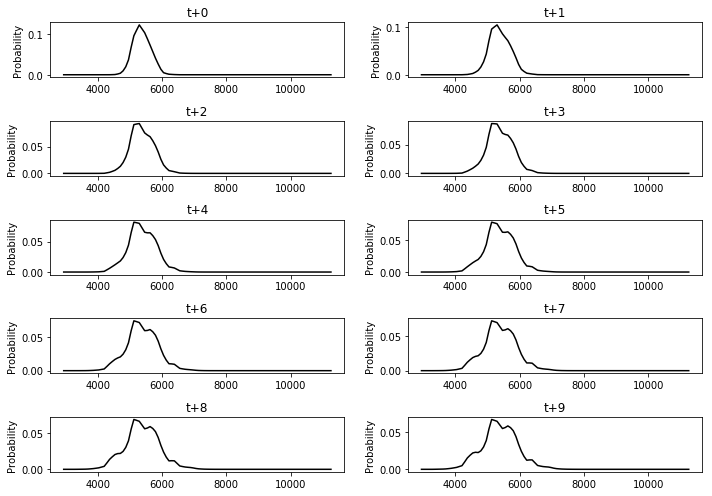
\includegraphics[width=\textwidth]{figures/pwfts_sample_manystep_tiled.png}
    \caption{Shapes of PWFTS probability distributions for many steps ahead forecasting}
    \label{fig:pwfts_sample_manystep_tiled}
\end{figure}

%%%%%%%%%%%%%%%%%%%%%%%%%%%%%%%%%%%%%%%%%%%%%%%%%%%%%%%%%%%%%%%%%%%%%%%%%%%%%%%%%%%%%%%
\subsection{High order models}
\label{sec:pwfts_high_order}

The PWFTS method described in Section \ref{sec:pwfts_training} is a first order method, i.e., it just needs $y(t)$ to forecast $\estimate$, while high order models use $\Omega$ time lags, whose indexes are stored on vector $L$. To extend the standard approach to high order  modification in Step 5 of the Training procedure is needed to adapt the FTPs and FTPGs to store $\Omega$ fuzzy sets on their LHS.

Once the fuzzyfied value $f(t)$ has multiple fuzzy sets (with different membership values greater than $alpha$-cut), a set of fuzzyfied values $f(t-L(\Omega)),...,f(t-L(0))$ must be represented with all possible combinations between the fuzzy sets of each lag, such as $f(t-L(\Omega)) \times f(t - L(\Omega-1)) \times \ldots \times f(t-L(0))$, where $\times$ represents the Cartesian Product operator. 

In Step 5 the FTPs will have the format $\ufset^{L(\Omega)}, \ufset^{L(\Omega-1)},\ldots,\ufset^{L(0)} \rightarrow A_i$, which can be read as ``IF $f(t-L(\Omega))$ is $\ufset^{L(\Omega)}$ AND $f(t-L(\Omega-1))$ is $\ufset^{L(\Omega-1)}$ AND $\dots$ AND $f(t-L(0))$ is $\ufset^{L(0)}$ THEN $f(t+1)$ is $A_i$". In Step 6, the high order FTPGs gather all high order FTPs with the same LHS. 

In Step 7 the $\pi_j$ weight is replaced by $\pi_{LHS}$ that aggregates the $\mu_{LHS}$ memberships of each FTPG for the samples. Given a sample $y(t-\Omega),\dots,y(t) \in Y$ with $\Omega$ lags, their membership grades with a FTPG is the product T-norm between all memberships of the LHS: 

\begin{equation}
\displaystyle  \mu_{LHS}(y(t-L(\Omega)),\ldots,y(t-L(0)) = \bigcap_{i = \Omega}^0 \mu_{\ufset}(y(t-L(i)))
\label{eqn:extension_highorder_mu}
\end{equation}

In the forecasting procedure, the Step 1 requires a sample with $\Omega$ lags that will generate $\Omega$ fuzzyfied values. In Step 2, all combinations between the fuzzy sets of each fuzzyfied lag will be the LHS of the affected PWFTPGs. In Step 3, in Equations \ref{eqn:pwfts_probabilistic}, \ref{eqn:pwfts_interval} and \ref{eqn:pwfts_point}, the empirical conditional probability $P(y(t)|A_i)$ will be replaced by $P(y(t-m),...,y(t) | LHS)$, the empirical conditional probability of the sample $y(t-m),...,y(t)$ given the LHS of the PWFTPG.

\begin{equation}
\displaystyle P(y(t-L(\Omega))\ldots y(t-L(0) | LHS) = \pi_{LHS} \frac{\mu_{LHS}(y(t-L(\Omega))\ldots,y(t-L(0))}{\sum_{\ufset \in LHS} Z_{\ufset}}
\label{eqn:extension_highorder}
\end{equation}


%%%%%%%%%%%%%%%%%%%%%%%%%%%%%%%%%%%%%%%%%%%%%%%%%%%%%%%%%%%%%%%%%%%%%%%%%%%%%%%%%%%%%%%
%%%%%%%%%%%%%%%%%%%%%%%%%%%%%%%%%%%%%%%%%%%%%%%%%%%%%%%%%%%%%%%%%%%%%%%%%%%%%%%%%%%%%%%

\section{Computational Experiments}
\label{sec:pwfts_experiments}

In this section presents an empirical study of the PWFTS performance using the same datasets, design of experiments and statistical tests employed in Sections \ref{sec:fts_experiments} and \ref{sec:prob_experiments}. PWFTS method can forecast points, intervals, and probability distributions, then the following sections will present all these compared results.

To measure the performance of the proposed models were chosen ARIMA, QAR, kNN/KDE, and BSTS as competitor models due to its possibility to perform point, interval and probabilistic forecasting for many steps ahead. The hyperparameters of each method were individually investigated and only the best model is taken account on the validation of the results. The HOFTS and WHOFTS methods were also used to compare the point forecasts, using the best models determined in Section \ref{sec:fts_experiments}. The $\ifts$ and $W\ifts$ methods were also used to compare the interval forecasts, and EnsembleFTS was also used to compare probabilistic forecasts, using the best models determined in Section \ref{sec:prob_experiments}.

In Section \ref{sec:pwfts_hyperparameters}, the accuracy sensitivity regarding to the hyperparameters of the proposed methods are analyzed using a grid search. The result of the experiments are presented in Sections \ref{sec:pwfts_experiments_point} for point forecasting, \ref{sec:pwfts_experiments_interval} for interval forecasting  and  \ref{sec:prob_experiments_probabilistic}, for probabilistic forecasting.

In order to contribute with the replication of all the results in the research, all data and source codes employed in this chapter are available at the URL:
\texttt{\url{http://bit.ly/scalable_probabilistic_fts_chap4}}

%%%%%%%%%%%%%%%%%%%%%%%%%%%%%%%%%%%%%%%%%%%%%%%%%%%%%%%%%%%%%%%%%%%%%%%%%%%%%%%%%%%%%%%
%%%%%%%%%%%%%%%%%%%%%%%%%%%%%%%%%%%%%%%%%%%%%%%%%%%%%%%%%%%%%%%%%%%%%%%%%%%%%%%%%%%%%%%
\subsection{Hyperparameter Grid Search}
\label{sec:pwfts_hyperparameters}

In order to asses the impact of the hyperparameters on PWFTS accuracy, a Search Grid was performed for each benchmark dataset, using the same search spaces contained on Table \ref{tab:ifts_gridsearch} of Section \ref{sec:prob_hyperparameters}. But, different from the previous experiments this grid search was performed for point, interval and probabilistic forecasting, in order to chose the hyperparameter values that best fit all cases.

The RMSE accuracy is shown on Figure \ref{fig:pwfts_gridsearch_point}, by order, number of partitions and dataset. The Winkler Score accuracy, where  $\alpha \in \{.05,.25\}$, can be observed on Figure \ref{fig:pwfts_gridsearch_interval} and the CRPS accuracy on Figure \ref{fig:pwfts_gridsearch_probabilistic}.

Once several numbers of partitions and order values achieved very closed accuracy values, the Principle of Parsimony (or Occam's Razor) was adopted to chose the set of hyperparameters that leads to smallest number of rules $|\model|$, keeping the same accuracy. The chosen hyperparameters were $k = 45$ and $\Omega = 1$ and a sample of the best models performance can be seen in Figure \ref{fig:pwfts_sample_onestep} (for one step ahead) and \ref{fig:pwfts_sample_manystep} (for many steps ahead).


\begin{figure}[htb]
    \centering
    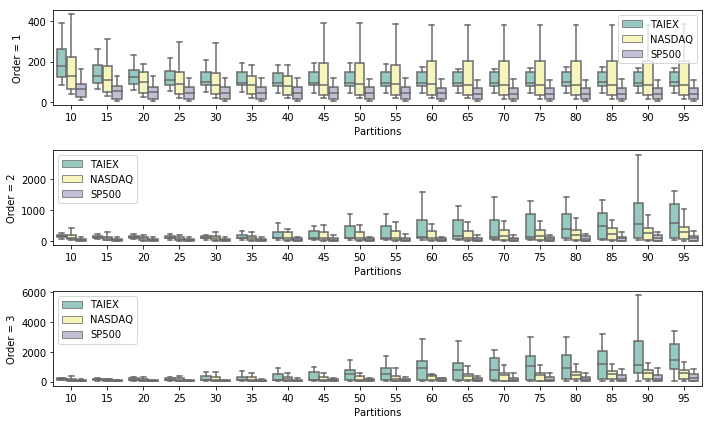
\includegraphics[width=\textwidth,height=12cm]{figures/pwfts_gridsearch_point.png}
    \caption{RMSE accuracy for order, partitions and dataset}
    \label{fig:pwfts_gridsearch_point}
\end{figure}

\begin{figure}[htb]
    \centering
    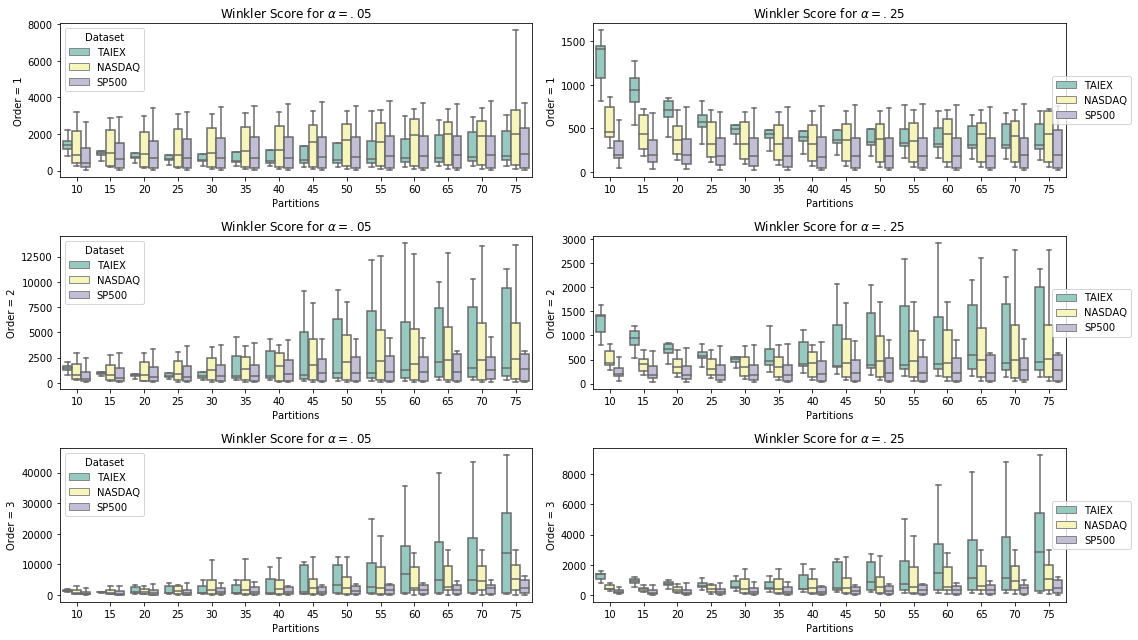
\includegraphics[width=\textwidth,height=12cm]{figures/pwfts_gridsearch_interval.png}
    \caption{Mean Winkler Score for $\alpha \in \{.05,.25\}$ by order, partitions and dataset}
    \label{fig:pwfts_gridsearch_interval}
\end{figure}

\begin{figure}[htb]
    \centering
    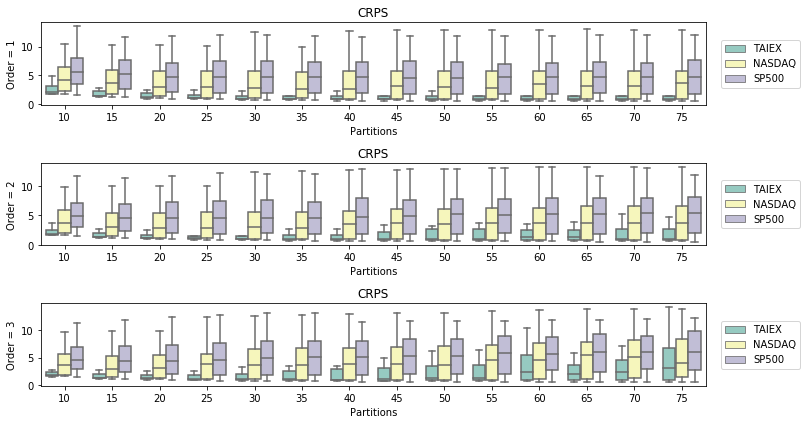
\includegraphics[width=\textwidth]{figures/pwfts_gridsearch_probabilistic.png}
    \caption{CRPS accuracy by order, partitions and dataset}
    \label{fig:pwfts_gridsearch_probabilistic}
\end{figure}


%%%%%%%%%%%%%%%%%%%%%%%%%%%%%%%%%%%%%%%%%%%%%%%%%%%%%%%%%%%%%%%%%%%%%%%%%%%%%%%%%%%%%%%
%%%%%%%%%%%%%%%%%%%%%%%%%%%%%%%%%%%%%%%%%%%%%%%%%%%%%%%%%%%%%%%%%%%%%%%%%%%%%%%%%%%%%%%
\subsection{Point Forecasting Benchmarks}
\label{sec:pwfts_experiments_point}

The RMSE results for each method and dataset are presented on Table \ref{tab:pwfts_point_results}. The Friedman Aligned Ranks of the methods are presented in Table \ref{tab:prob_interval_ranks} and the test statistic for these results is $Q = 13.903114186851207$, where the p-value is $P(\chi^2_{df} < Q) = 0.030737356514312197$, with $df=7$ degrees of freedom. For this statistic the $H_0$ is rejected at the $\alpha=.05$ confidence level, indicating that there is difference between the means of the competitor models.

The \textit{post-hoc} tests were employed using PWFTS as control methods and their results are presented on Table \ref{tab:pwfts_point_posthoc}, showing that there is no prevalence of PWFTS method over all others. The mean difference detected by the Friedman Test occurred between QAR and BSTS, where QAR prevails over BSTS with p-value of 0.006984, rejecting $H_0$ of \textit{post-hoc} tests. These results showed that PWFTS point forecasting method perform satisfactorily when compared with the standard methods in the literature. 

The statistical tests were employed to one step ahead forecasts. Figure \ref{fig:pwfts_ahead_point} shows, for each method and dataset, the impact of the forecasting horizon on the RMSE accuracy.

\begin{table}[ht]
\resizebox{\textwidth}{!}{% <------ Don't forget this %
\centering
    \begin{tabular}{|c|ccccccc|}
\hline
\textbf{Dataset} & \textbf{ARIMA} & \textbf{QAR} & \textbf{PWFTS} & \textbf{WHOFTS} & \textbf{HOFTS} & \textbf{kNN} & \textbf{BSTS} \\
\hline
\multirow{2}{*}{S\&P 500} &     6.091 &     8.177 &    10.541 &    12.822 &    13.605 &    19.242 &    380.466 \\
 &   $\pm$7.452 &  $\pm$11.366 &   $\pm$10.19 &  $\pm$11.336 &  $\pm$12.392 &   $\pm$24.97 &  $\pm$947.809 \\ \hline
\multirow{2}{*}{NASDAQ} &    22.592 &    17.951 &    24.839 &    27.154 &    29.713 &    34.742 &    413.494 \\
 &  $\pm$24.991 &  $\pm$11.965 &  $\pm$18.198 &   $\pm$15.05 &  $\pm$12.875 &  $\pm$25.096 &  $\pm$837.281 \\ \hline
\multirow{2}{*}{TAIEX} &    91.311 &      66.9 &    75.558 &    90.433 &   100.787 &    80.213 &     271.66 \\
 &  $\pm$63.249 &  $\pm$44.369 &  $\pm$56.739 &   $\pm$58.93 &  $\pm$62.932 &  $\pm$56.494 &  $\pm$250.078 \\ \hline
\end{tabular}
}
    \caption{RMSE for one step ahead point forecasts}
    \label{tab:pwfts_point_results}
\end{table}

\begin{table}[hbt]
    \centering
    \begin{tabular}{|c|c|}
\hline
       METHOD &       RANK \\
\hline
QAR &   6.333333 \\
ARIMA &   7.333333 \\
PWFTS &   8.333333 \\
WHOFTS &  10.333333 \\
HOFTS &  12.000000 \\
kNN &  12.666667 \\
BSTS &  20.000000 \\
\hline
\end{tabular}
    \caption{Friedman aligned ranks for point forecasts}
    \label{tab:pwfts_point_ranks}
\end{table}

\begin{table}[htb]
\resizebox{\textwidth}{!}{% <------ Don't forget this %
    \centering
    \begin{tabular}{llrrrl}
\toprule
{} &       COMPARISON &   Z-VALUE &   P-VALUE &  ADJUSTED P-VALUE &       Result \\
\midrule
0 &    PWFTS vs BSTS &  2.302831 &  0.021288 &          0.121122 &  H0 Accepted \\
1 &     PWFTS vs kNN &  0.855337 &  0.392364 &          0.775648 &  H0 Accepted \\
2 &   PWFTS vs HOFTS &  0.723747 &  0.469221 &          0.775648 &  H0 Accepted \\
3 &     PWFTS vs QAR &  0.394771 &  0.693012 &          0.829909 &  H0 Accepted \\
4 &  PWFTS vs WHOFTS &  0.394771 &  0.693012 &          0.829909 &  H0 Accepted \\
5 &   PWFTS vs ARIMA &  0.197386 &  0.843526 &          0.843526 &  H0 Accepted \\
\bottomrule
\end{tabular}
}
    \caption{Post-hoc tests using PWFTS as control method}
    \label{tab:pwfts_point_posthoc}
\end{table}

\begin{figure}[htb]
    \centering
    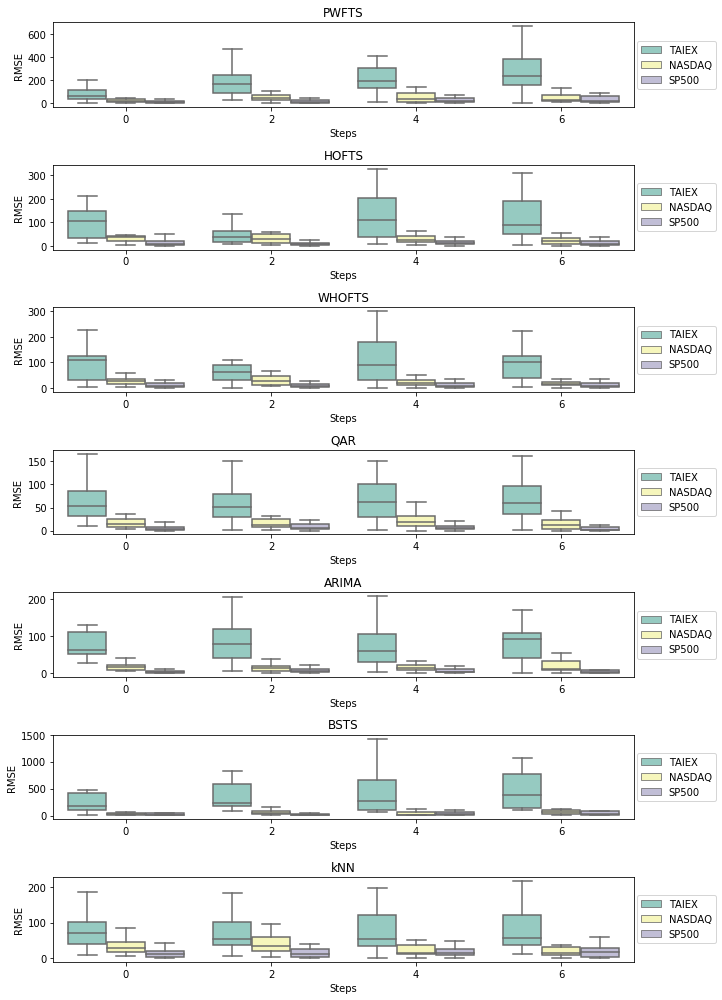
\includegraphics[width=\textwidth]{figures/pwfts_ahead_point.png}
    \caption{Impact of the forecasting horizon on RMSE accuracy}
    \label{fig:pwfts_ahead_point}
\end{figure}

%%%%%%%%%%%%%%%%%%%%%%%%%%%%%%%%%%%%%%%%%%%%%%%%%%%%%%%%%%%%%%%%%%%%%%%%%%%%%%%%%%%%%%%
%%%%%%%%%%%%%%%%%%%%%%%%%%%%%%%%%%%%%%%%%%%%%%%%%%%%%%%%%%%%%%%%%%%%%%%%%%%%%%%%%%%%%%%
\subsubsection{Residual Analysis}
\label{sec:pwfts_residual}

The residuals of the models are presented in Figures \ref{fig:pwfts_residual} and the Ljung-Box tests for the 3 first lags are presented in Table \ref{tab:pwfts_residual} , which is shown the good fit of the model. 

\begin{figure}[h]
    \centering
    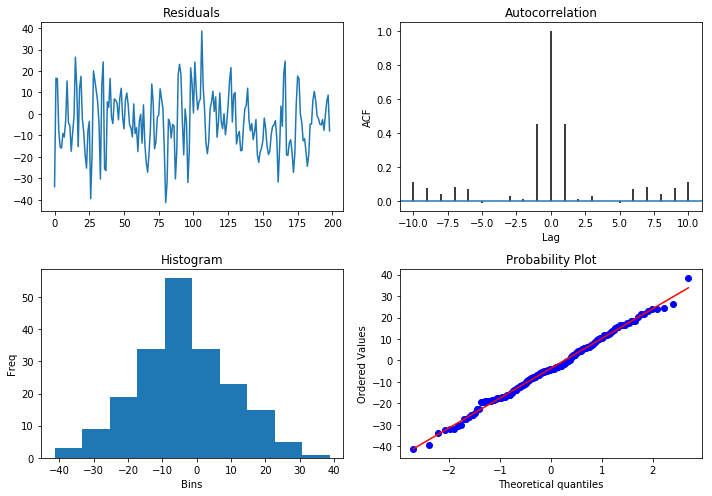
\includegraphics[width=\textwidth,height=7cm]{figures/pwfts_residual.png}
    \caption{Residual analysis of PWFTS}
    \label{fig:pwfts_residual}
\end{figure}

\begin{table}[htb]
    \centering
\begin{tabular}{lrrrrl}
\toprule
Lag &  Statistic &       p-Value &  Critical Value &       Result \\
\midrule
1 &  34.846143 &  3.568157e-09 &        3.841459 &  H0 accepted \\
2 &  35.497255 &  1.958254e-08 &        5.991465 &  H0 accepted \\
3 &  35.871542 &  7.971605e-08 &        7.814728 &  H0 accepted \\
\bottomrule
\end{tabular}
    \caption{Ljung-Box Test for the 3 first lags}
    \label{tab:pwfts_residual}
\end{table}

%%%%%%%%%%%%%%%%%%%%%%%%%%%%%%%%%%%%%%%%%%%%%%%%%%%%%%%%%%%%%%%%%%%%%%%%%%%%%%%%%%%%%%%
%%%%%%%%%%%%%%%%%%%%%%%%%%%%%%%%%%%%%%%%%%%%%%%%%%%%%%%%%%%%%%%%%%%%%%%%%%%%%%%%%%%%%%%
\subsection{Interval Forecasting Benchmarks}
\label{sec:pwfts_experiments_interval}

The Winkler Score Mean results for each method and dataset are presented on Table \ref{tab:pwfts_interval_results}. The Friedman Aligned Ranks of the methods are presented in Table \ref{tab:pwfts_interval_ranks} and the test statistic for these results is $Q = 14.812664$, where the p-Value is $P(\chi^2_{df} < Q) = 0.038477$, with $df=7$ degrees of freedom. For this statistic, the $H_0$ is rejected at the $\alpha=.05$ confidence level, indicating that there is a difference between the means of the competitor models.

The \textit{post-hoc} tests were employed using PWFTS as control methods and their results are presented in Table \ref{tab:pwfts_interval_posthoc}, showing the prevalence of PWFTS over BSTS. These results showed that PWFTS interval forecasting methods perform satisfactorily when compared with other standard methods in the literature. 

The statistical tests were employed on the one-step ahead forecasts. Figure \ref{fig:pwfts_ahead_interval} shows, for each dataset, the impact of the forecasting horizon on the Winkler Score accuracy of PWFTS.


\begin{table}[h]
\resizebox{\textwidth}{!}{% <------ Don't forget this %
\centering
\begin{tabular}{|c|cccccccc|}
\hline
\textbf{Dataset} & \textbf{ARIMA} & \textbf{PWFTS} & \textbf{QAR} & \textbf{WIFTS} & \textbf{IFTS} & \textbf{kNN} & \textbf{EnsembleFTS} & \textbf{BSTS} \\ \hline
\multirow{2}{*}{S\&P 500} &      72.712 &    73.505 &    121.694 &    111.705 &    113.516 &    131.394 &     268.567 &     292.415 \\
 &   $\pm$135.871 &   $\pm$99.09 &  $\pm$319.305 &  $\pm$156.013 &   $\pm$91.627 &   $\pm$166.31 &   $\pm$318.259 &   $\pm$384.499 \\ \hline
\multirow{2}{*}{NASDAQ} &     233.261 &   112.944 &    106.416 &     123.35 &    284.692 &    170.709 &     603.881 &     652.036 \\
 &   $\pm$486.735 &  $\pm$33.666 &   $\pm$56.248 &  $\pm$141.251 &   $\pm$147.24 &  $\pm$156.097 &   $\pm$638.297 &   $\pm$963.624 \\ \hline
\multirow{2}{*}{TAIEX} &     858.124 &   348.647 &        340 &    480.581 &    917.879 &    428.484 &     898.531 &     1280.67 \\
 &  $\pm$1337.139 &  $\pm$82.036 &   $\pm$269.34 &  $\pm$561.826 &  $\pm$243.737 &  $\pm$269.459 &  $\pm$1175.107 &  $\pm$1472.031 \\ \hline
\end{tabular}
}
    \caption{Average Winkler Score with $\alpha=.05$ for one step ahead interval forecasts}
    \label{tab:pwfts_interval_results}
\end{table}

\begin{table}[hbt]
    \centering
    \begin{tabular}{|c|c|}
\hline
       METHOD &       RANK \\
\hline
PWFTS &   6.000000 \\
QAR &   6.666667 \\
WIFTS &   7.666667 \\
kNN &   8.666667 \\
ARIMA &  13.000000 \\
IFTS &  16.666667 \\
EnsembleFTS &  19.666667 \\
BSTS &  21.666667 \\
\hline
\end{tabular}
    \caption{Friedman aligned ranks for interval forecasts }
    \label{tab:pwfts_interval_ranks}
\end{table}

\begin{table}[htb]
\resizebox{\textwidth}{!}{% <------ Don't forget this %
    \centering
\begin{tabular}{llrrrl}
\toprule
{} &            COMPARISON &   Z-VALUE &   P-VALUE &  ADJUSTED P-VALUE &       Result \\
\midrule
0 &         PWFTS vs BSTS &  2.713546 &  0.006657 &          0.045677 &  H0 Rejected \\
1 &  PWFTS vs EnsembleFTS &  2.367136 &  0.017926 &          0.061349 &  H0 Accepted \\
2 &         PWFTS vs IFTS &  1.847521 &  0.064672 &          0.144442 &  H0 Accepted \\
3 &        PWFTS vs ARIMA &  1.212436 &  0.225346 &          0.360355 &  H0 Accepted \\
4 &          PWFTS vs kNN &  0.461880 &  0.644167 &          0.764634 &  H0 Accepted \\
5 &        PWFTS vs WIFTS &  0.288675 &  0.772830 &          0.822550 &  H0 Accepted \\
6 &          PWFTS vs QAR &  0.115470 &  0.908073 &          0.908073 &  H0 Accepted \\
\bottomrule
\end{tabular}
}
    \caption{Post-hoc tests using PWFTS as control method}
    \label{tab:pwfts_interval_posthoc}
\end{table}

\begin{figure}[htb]
    \centering
    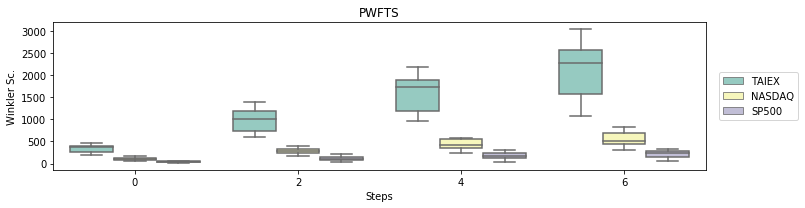
\includegraphics[width=\textwidth]{figures/pwfts_ahead_interval.png}
    \caption{Impact of the forecasting horizon on Winkler Score accuracy}
    \label{fig:pwfts_ahead_interval}
\end{figure}

%%%%%%%%%%%%%%%%%%%%%%%%%%%%%%%%%%%%%%%%%%%%%%%%%%%%%%%%%%%%%%%%%%%%%%%%%%%%%%%%%%%%%%%
%%%%%%%%%%%%%%%%%%%%%%%%%%%%%%%%%%%%%%%%%%%%%%%%%%%%%%%%%%%%%%%%%%%%%%%%%%%%%%%%%%%%%%%
\subsection{Probabilistic Forecasting Benchmarks}
\label{sec:pwfts_experiments_probabilistic}

The CRPS Mean results for each method and dataset are presented in Table \ref{tab:pwfts_probabilistic_results}. The Friedman Aligned Ranks of the methods are presented in Table \ref{tab:pwfts_probabilistic_ranks} and the test statistic for these results is $Q = 10.352711804324706$, where the p-Value is $P(\chi ^2_{df} < Q) = 0.06583635032195168$, with $df=5$ degrees of freedom. For this statistic the $H_0$ is accepted at the $\alpha = .05$ confidence level, indicating that there is no significant difference between the means of the competitor models. This result discards the need to employ \textit{post-hoc} tests and show that there is no prevalence of one method over others, showing also that PWFTS probabilistic forecasting method performed satisfactorily when compared with the standard methods in the literature. 

The statistical tests were employed on the one-step ahead forecasts. Figure \ref{fig:pwfts_ahead_probabilistic} shows, for each dataset, the impact of the forecasting horizon on the CRPS accuracy of PWFTS method.

\begin{table}[h]
\resizebox{\textwidth}{!}{% <------ Don't forget this %
\centering
\begin{tabular}{|c|cccccc|}
\hline
\textbf{Dataset} & \textbf{PWFTS} & \textbf{QAR} & \textbf{kNN} & \textbf{ARIMA} & \textbf{EnsembleFTS} & \textbf{BSTS} \\
\hline
\multirow{2}{*}{NASDAQ} &    0.882 &    1.028 &    1.158 &    1.444 &       1.923 &    3.208 \\
 &  $\pm$0.347 &  $\pm$0.748 &  $\pm$0.477 &  $\pm$1.303 &     $\pm$1.416 &  $\pm$3.983 \\ \hline
\multirow{2}{*}{TAIEX} &    0.967 &    1.135 &    1.229 &    1.691 &       1.301 &    4.081 \\
 &  $\pm$0.404 &  $\pm$0.613 &  $\pm$0.693 &  $\pm$1.239 &     $\pm$1.118 &  $\pm$5.306 \\ \hline
\multirow{2}{*}{S\&P 500} &    1.257 &    1.557 &    4.403 &    1.216 &       1.995 &    3.278 \\
 &  $\pm$0.722 &   $\pm$1.74 &  $\pm$3.261 &  $\pm$1.166 &     $\pm$2.255 &   $\pm$3.16 \\ \hline
\end{tabular}
}
    \caption{CRPS for one step ahead interval forecasts}
    \label{tab:pwfts_probabilistic_results}
\end{table}

\begin{table}[hbt]
    \centering
    \begin{tabular}{|c|c|}
\hline
       METHOD &       RANK \\
\hline
PWFTS &   3.333333 \\
QAR &   5.666667 \\
ARIMA &   8.666667 \\
kNN &  11.333333 \\
EnsembleFTS &  11.666667 \\
BSTS &  16.333333 \\
\bottomrule
\end{tabular}
    \caption{Friedman aligned ranks for probabilistic forecasts }
    \label{tab:pwfts_probabilistic_ranks}
\end{table}

\begin{figure}[htb]
    \centering
    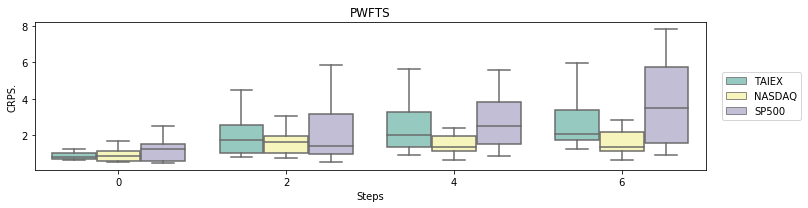
\includegraphics[width=\textwidth]{figures/pwfts_ahead_probabilistic.png}
    \caption{Impact of the forecasting horizon on CRPS accuracy}
    \label{fig:pwfts_ahead_probabilistic}
\end{figure}

%%%%%%%%%%%%%%%%%%%%%%%%%%%%%%%%%%%%%%%%%%%%%%%%%%%%%%%%%%%%%%%%%%%%%%%%%%%%%%%%%%%%%%%
%%%%%%%%%%%%%%%%%%%%%%%%%%%%%%%%%%%%%%%%%%%%%%%%%%%%%%%%%%%%%%%%%%%%%%%%%%%%%%%%%%%%%%%
\section{Conclusion}
\label{sec:pwfts_conclusion}

This chapter proposed a new univariate and time invariant FTS method - the Probabilistic Weighted FTS (PWFTS), a weighted rule-based FTS method which represents their temporal patterns with an empirical probability - based on the proposed concept of fuzzy frequency. The PWFTS rule model - the Probabilistic Weighted Fuzzy Temporal Pattern Groups (PWFTPG) - describes fuzzy and stochastic behavior of time series and combines them to produce forecasts. 

Once was already proposed interval and probabilistic methods, none of them integrate all these capabilities. The strength of PWFTS is its flexibility and performance. This model is used to produce probability densities, prediction intervals and point forecasting, with high order models and multiple-step ahead forecasting.  

Computational experiments were performed to evaluate the accuracy of the proposed model which showed equivalent or better performance than standard methods on literature. Its computational cost is low when compared with BSTS and EnsembleFTS approaches and its interval accuracy is better than WIFTS and IFTS.

The proposed PWFTS method extends FTS methods to deal with interval and probabilistic forecasting applications, which is the major contribution of this research. Moreover, PWFTS improves on former FTS methods in the literature by considering the concept of fuzzy frequency and empirical probabilities in the generation of the rule knowledge base. The proposed method improves previous FTS methods by aggregating probabilistic and interval forecasting capabilities into a single model, being useful for a wide range of applications and user needs.

\subsection{Method limitations}

As in previous FTS methods, the PWFTS accuracy depends on the hyperparameter fine tunning. The method does not embody this optimization and it is advisable that this fine tunning be performed. Another issue about the model optimization is the parsimony: PWFTS weights may vanish as the number of rules increases. The weights precision is limited by the computational numerical precision. 

In general all forecasting procedures are computationally cheap but the probabilistic forecasting for multiple-steps ahead is computationally expensive and the forecasting horizon H must be chosen carefully.
